% Fig 3.21 Muonium atom: a positive muon (mu+) with an electron (e-) orbiting it.
\documentclass[tikz,border=5pt]{standalone}
\usetikzlibrary{arrows.meta}
\usepackage{amsmath}
\usepackage{bm}
\usepackage{fontspec}
\setmainfont{Times New Roman}
\begin{document}
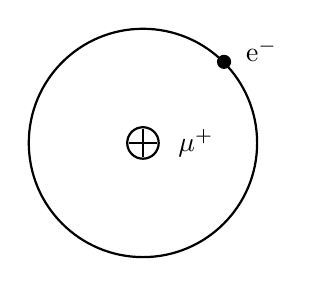
\begin{tikzpicture}[line width=0.8pt,>=Stealth]
% electron orbit
\draw (1.7,1.7) circle (1.45);
% positive muon at the centre (circled plus)
\draw (1.7,1.7) circle (0.20);
\draw (1.52,1.7) -- (1.88,1.7);
\draw (1.7,1.52) -- (1.7,1.88);
\node[anchor=west] at (2.02,1.70) {$\mu^+$};
% electron on the orbit (upper right)
\fill (2.73,2.73) circle (0.09);
\node[anchor=west] at (2.88,2.88) {e$^-$};
\end{tikzpicture}
\end{document}
